% This file was created with tikzplotlib v0.10.1.
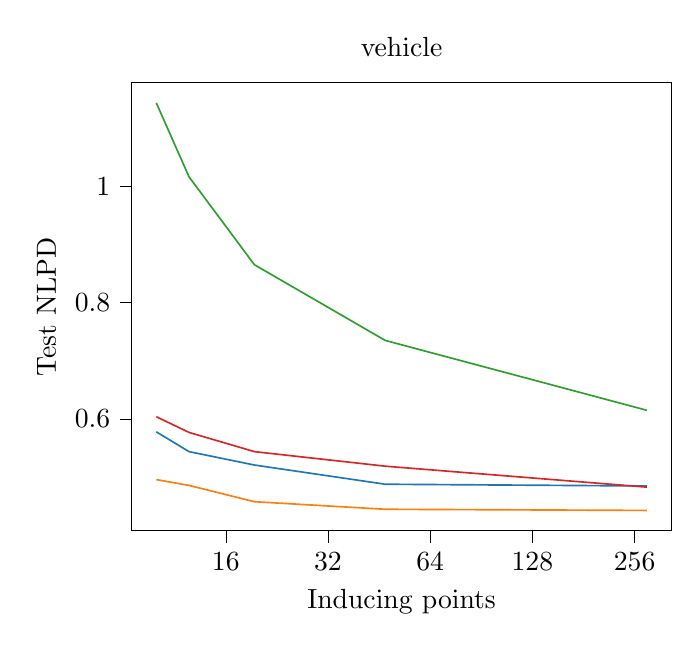
\begin{tikzpicture}

\definecolor{crimson2143940}{RGB}{214,39,40}
\definecolor{darkgray176}{RGB}{176,176,176}
\definecolor{darkorange25512714}{RGB}{255,127,14}
\definecolor{forestgreen4416044}{RGB}{44,160,44}
\definecolor{steelblue31119180}{RGB}{31,119,180}

\begin{axis}[
tick align=outside,
tick pos=left,
title={vehicle},
x grid style={darkgray176},
xlabel={Inducing points},
xmin=4, xmax=268,
xtick style={color=black},
xtick={0,50,100,150,200,250,300},
xticklabels={0,16,32,64,128,256,},
y grid style={darkgray176},
ylabel={Test NLPD},
ymin=0.408, ymax=1.178,
ytick style={color=black}
]
\addplot [semithick, steelblue31119180]
table {%
16 0.578
32 0.544
64 0.521
128 0.488
256 0.485
};
\addplot [semithick, darkorange25512714]
table {%
16 0.496
32 0.486
64 0.458
128 0.445
256 0.443
};
\addplot [semithick, forestgreen4416044]
table {%
16 1.143
32 1.016
64 0.865
128 0.735
256 0.615
};
\addplot [semithick, crimson2143940]
table {%
16 0.604
32 0.577
64 0.544
128 0.519
256 0.483
};
\end{axis}

\end{tikzpicture}
